\chapter{Users Interaction Structure}
\section{Interaction Structure}
We next study the patterns of member engagements with listeners on 7cot. 
The patterns are found through analysis of a network where members and listeners
are connected if they held at least one conversation with each other. 
We also study networks that connect members (listeners) 
to each other if they had a conversation with at least one common listener
(member).  Structural analyses of the networks inform how members are 
choosing to engage with listeners on 7cot, if some subsets of listeners
are more popular than others, and if a pattern of members selectively 
choosing listeners can be seen.

\begin{figure}
	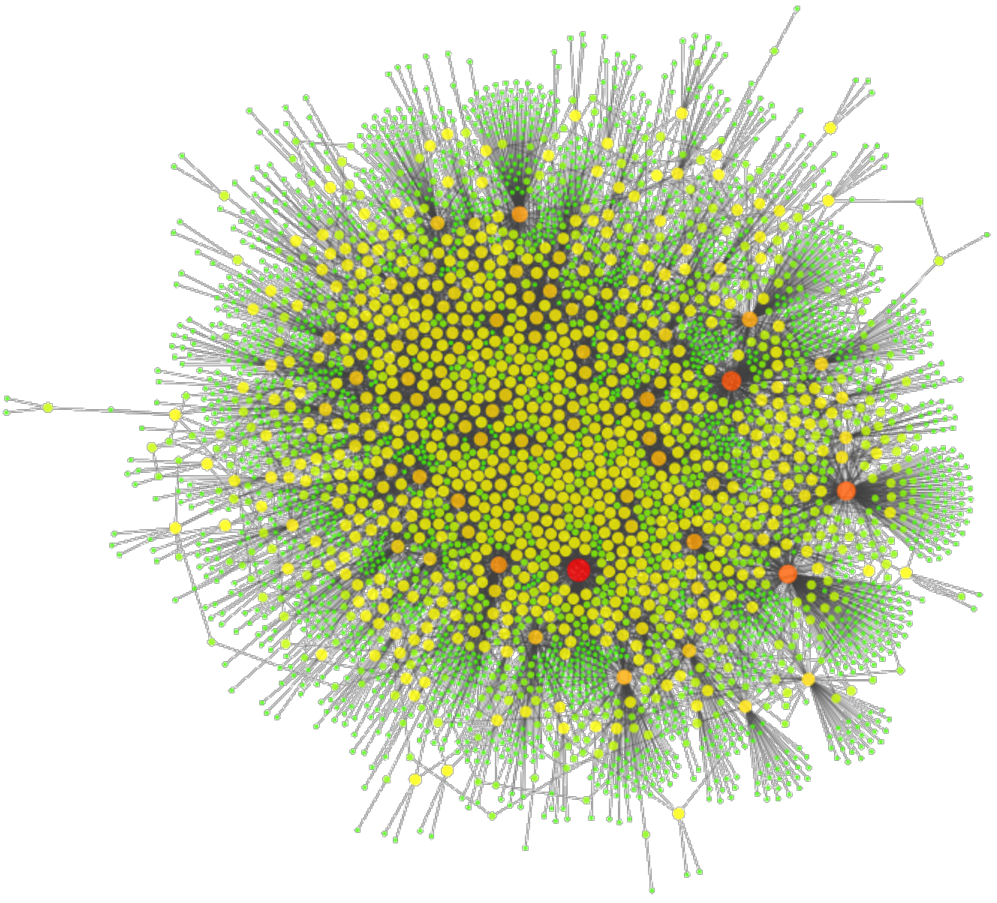
\includegraphics[width=\textwidth]{bpn.pdf}
	\caption{7cot bipartite network; listeners are green and members are colored with 
		hotter colors by their degree.}
	\label{fig:bpn}
\end{figure}

We represent all 7cot interactions as a bipartite network from members to listeners.
We consider all conversations that contained 
at least one message sent by either a member or listener (note that guests are excluded
from this analysis and will be the subject of future work). Figure~\ref{fig:bpn}
illustrates the structure of this bipartite network. Here, listeners are colored green while
member nodes are sized larger and colored hotter by their degree. The coloring finds a 
presence of some members that connect to vast numbers of other listeners, while the majority
of members connect to a similar number. Moreover, we note that green nodes in the 
center of the network represent listeners who are embedded between a large number of other
members, while listeners at the periphery of the network only connect to a very small number
of others. The ratio of embedded to periphery nodes in the structure may indicate that most
listeners go underutilized or simply choose to connect to a small number of others. 
Table~\ref{tab:proj} lists the structural features of this bipartite 
network. The network has an average degree $\langle k \rangle$ of $5.39$, 
i.e. members tend to connect to between five or six distinct listeners
during their time on the service. 
%% Rev
This reaffirms the idea that members seek help from a number of others, perhaps
to obtain different viewpoints or thoughts about their emotional problem. 
%We also visualize
%the entire bipartite network in Figure~\ref{fig:bpn} and color and size members by their
%degree. It illustrates how there are a sizeable number of `overactive' that connect
%to a particularly large, possibly abnormal number of listeners.
We also computed
the number of connected components in the network. Only 477 disconnected components exist,
the largest of which (GCC) includes virtually every user (99.2\%) on the platform.
%Rev
In other words, there are virtually no members or listeners on 7cot who choose to 
exclusively search for and communicate only with each other. 
The single large GCC lets us compute the average path length in the network as
$\bar{d} = \log(|V|/z_1)/\log(z_2/z_1) + 1$, an expression valid for 
networks that are nearly fully connected~\cite{newman2010networks}, 
where $z_1$ and $z_2$ are the average number of others a user can reach within
one and two hops respectively. The small average path length $\bar{d} = 3.46$
may be indicative of the existence of a large `core' of members and 
listeners serving as hubs that connect members and listeners to others across
the bipartite structure. 
%%Rev
Listeners in the `core' may thus connect to large and diverse sets of members, i.e., 
are the listeners that connect to members who request to speak with 
any available listener. 

\begin{table}
	\setlength\extrarowheight{0.5pt}
	\begin{tabular}{r| c | c | c}
		& Bipartite Network & Member Proj. & Listener Proj. \\
		\hline
		$|V|$ & 117,372 & 86,877 & 30,495 \\
		$|E|$ & 465,437 & 12,657,611 & 10,359,604 \\
		$\langle k \rangle$ & 5.39 & 291.39 & 679.43 \\
		$\mathcal{C}$ & N/A & 0.734 & 0.636 \\ %0.22
		$\mathcal{A}$ & N/A & -0.10 & -0.06 \\
		$\bar{d}$ & 3.46 & 2.56 & 2.30 \\
		$\rho$ & N/A & 0.003 & 0.022 \\ %0.0002
		Components & 447 & 447 & 447 \\
		GCC Size & 116,411 (99.2\%) & 86,364 (99.4\%) & 30,047 (98.5\%) \\
	\end{tabular}
	\caption{Bipartite and projection network features}
	
	\label{tab:proj}
\end{table}

We omit measuring the clustering coefficient $\mathcal{C}$, degree
assortativity $\mathcal{A}$, and density $\rho$ of bipartite network because their 
definitions are closely related to measurements taken over the network's
{\em one-mode projections}~\cite{guillaume2006bipartite}.
One-mode projections capture the structure of 
interaction co-occurrences among the $g$ listeners and $n$ members
of 7cot.
Given a matrix $\mathbf{B} \in \mathbb{R}^{g \times n}$ where 
$\mathbf{B}_{ij} = 1$ if listener $i$ has a conversation
with member $j$, we define $\mathbf{P}^{(m)} = \mathbf{B}^T\mathbf{B} \in \mathbb{R}^{n \times n}$ and 
$\mathbf{P}^{(l)} = \mathbf{B}\mathbf{B}^T \in \mathbb{R}^{g \times g}$ as the adjacency matrices 
of the member and listener projection networks, respectively. We then have $\mathbf{P}^{(m)}_{ij} = c$ 
($\mathbf{P}^{(l)}_{ij} = c$)
if members (listeners) $i$ and $j$ hold a conversation 
with $c$ common listeners (members). Structural patterns within the
projection networks are discussed next. 

\begin{figure}
	\subfloat[Member network sample]{\includegraphics[width=0.45\textwidth]{ccvismem.pdf}%
		\label{fig:memsample}}
	\hfill
	\subfloat[Listener network sample]{\includegraphics[width=0.45\textwidth]{ccvislist.pdf}%
		\label{fig:listsample}}
	\caption{Edge sampled projection networks with nodes colored by clustering coefficient}
	\label{fig:sample}
	
\end{figure}

\subsection{Connectivity patterns}
Table~\ref{tab:proj} gives the mean degree, global clustering coefficient, degree assortativity, average path length, 
density, and GCC size of the member and listener projection networks. 
These statistics may be compared with a visualization of a random sampling~\cite{ahmed2014network} of 
10,000 edges of the projection networks in Figure~\ref{fig:sample}. 
Nodes are colored hotter in the figure if they 
have a higher local clustering coefficient $\mathcal{C}_l$ 
(green nodes have $\mathcal{C}_l = 0$ and red nodes have $\mathcal{C}_l = 1$) 
and are 
drawn under a force directed layout so that nodes separated by small
distances are positioned closer together. 
Although sophisticated sampling algorithms are needed to create samples that maintain many
structural features of the sampled network~\cite{doran2014triad}, edge sampling still conveys the shape
of the global network within the interconnected core of the sample
(nodes participating in excessive numbers of open triangles are likely an artifact
of edge sampling).  
The high mean degree, large GCC size, and small average path lengths of both projections further
support the hypothesis that members and listeners do not limit themselves to interact 
with a small subset of listeners (members). They both exhibit weak negative degree 
assortativity, suggesting a small inclination
for members (listeners) who share just a few common listeners (members) with others share
them with those who have large numbers of listeners (members) in common with others.
However, the lower degree, larger clustering
coefficient, and larger path lengths of the member network imply a weak penchant for members 
to form clusters by the common listeners they connect to. Such clusters
can be seen in Figure~\ref{fig:memsample} as cliques in the core of 
the member network. 
%%Ref
These clusters may be traces of member groups that connect to similar `types' of listeners. 
\begin{figure}[t]
	\subfloat[Member projection]{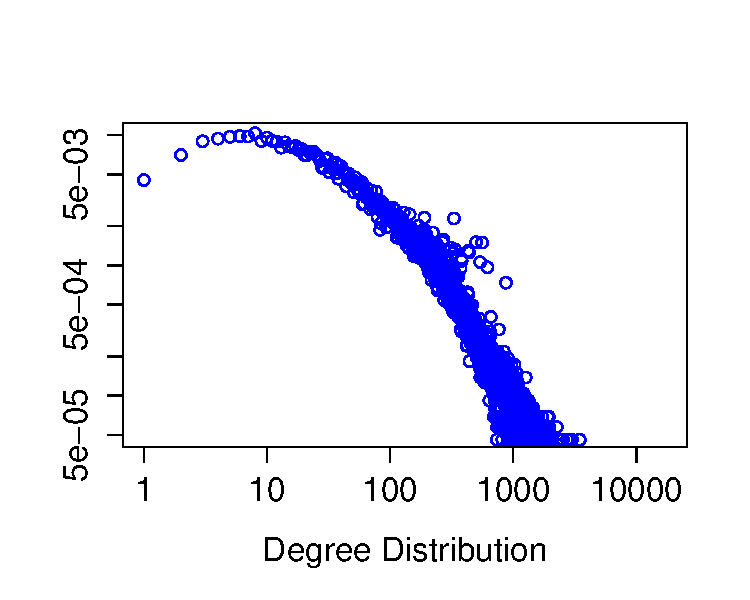
\includegraphics[width=0.45\textwidth]{ddmem.pdf}%
		\label{fig:ddmem}}
	\hfill
	\subfloat[Listener projection]{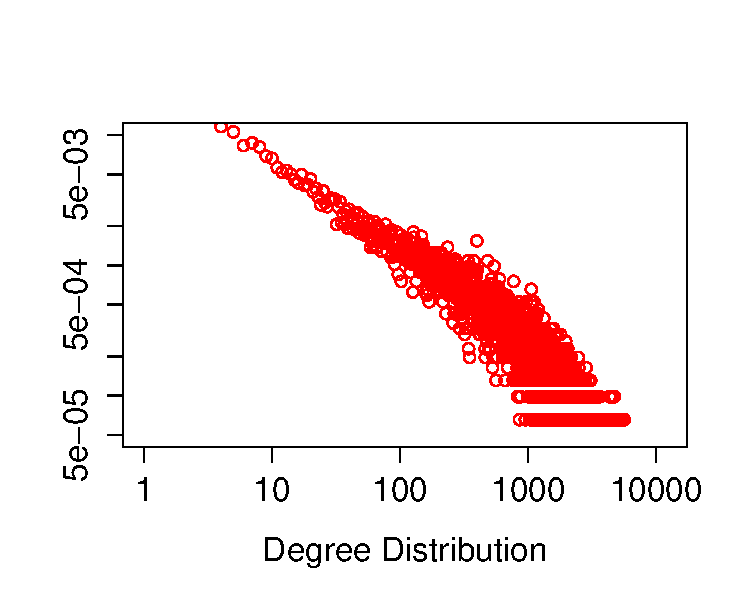
\includegraphics[width=0.45\textwidth]{ddlist.pdf}%
		\label{fig:ddlist}}
	\caption{Projection network degree distributions}
	\label{fig:dd}
\end{figure}

We find the degree distributions of the projection networks, presented in log-log
scale in Figure~\ref{fig:dd}, to take dissimilar shapes. The listener degree
distribution exhibits a near straight line pattern
indicative of a power-law distribution, but the  pattern is less pronounced 
in the member degree distribution. 
We quantify this difference by running a maximum likelihood based test of the null hypothesis 
{\em $H_0$: the empirical data has a power-tailed distribution} (the test also yields
best fitting power-law exponent $\alpha$ under the null)~\cite{clauset2009power}.
The test leaves little room to reject $H_0$ for the listener degree distribution 
($p = 0.985; \alpha = 2.51$). However, there is more doubt for
the member degree distribution ($p = 0.362; \alpha = 2.34$). 
That the listener degree distribution has a
power-tail suggests significant variation in the number of common members listeners share
with each other, and that the probability of sharing orders of magnitude more members than
expected is not negligible. A similar statement could be made about members, however 
they may exhibit less variation since we are less confident if a power-tailed trend exists. 
%Rev
The difference of the distributions shape may be explained by members who only need to connect to a limited
number of listeners in order to have many problems resolved, or by members who choose to 
connect deeply with a small number of listeners. Such behaviors place
a `soft limit' on the largest number of listeners members may connect to, weakening the support for a 
power-tail to emerge~\cite{lipsky2008queueing}.  On the other hand, so long as a listener is available for 
newly added members to connect to, there may be no limit on the number of 
new members a listener may connect to over time.

\subsection{Centrality analysis}
We also study connectivity-based notions of network centrality in the 
projection networks. We first consider the betweenness centrality
of a user $u$, defined as 
$b(u) = \sum_{u\neq i \neq j} \sigma_{ij}(u) / \sigma_{ij}$ where 
$\sigma_{ij}$ is the number of shortest paths from users $i$ to $j$ and
$\sigma_{ij}(u)$ is the number of such paths that include $u$. 
This measure reflects the notion that a user is `central' if she is often part of the 
shortest path among two others in the network. Figure~\ref{fig:btcdf}
plots the cumulative distribution (CDF) of the centrality scores across the 
two networks on semi-log scale. Its rapid ascent and long left tail
indicate that almost all users are part of a number of shortest paths in the network. 
The networks are therefore structurally robust to the loss of users. 
%%Rev
%In other words,
%clusters of members that prefer similar `types' of listeners may not be exclusive
%to just one user type. 
We also consider the closeness centrality of a user $u$,
defined as $c(u) = (\sum_{j} d(u,j))^{-1}$ where $d(u,j)$ is the distance
from user $u$ to $j$. Figure~\ref{fig:clcdf} gives the CDF of closeness centrality
on the two networks (note that the $x$-axis is not in log scale). That the
CDF for the listener distribution is stretched farther than the 
member distribution is only because there are fewer nodes in the network.
Unlike betweenness centrality, the closeness centrality CDF 
of the two networks takes on different shapes. 
The CDF of the member network has only a slight
curvature at its left and right tail, with a nearly linear body. This suggests
that the centrality scores exhibit a small peak around
the mean of the distribution but are otherwise uniformly distributed.
The centrality scores of listeners are uniformly distributed up to 
approximately the $40^{th}$ percentile, at which point they become
heavily skewed. A majority of listeners, therefore, 
are at a much shorter distance from those below this $40^{th}$ percentile.
%%Rev
This pattern may be indicative of a core-periphery structure~\cite{rombach2014core}
in the listener projection network that does not exist in the member one, 
where those in the core (periphery) have high (low) closeness centrality. 
The probability of a listener falling in the core may be correlated with the 
diversity of the members she connects to: connecting to many different
members increases the probability of sharing a connection with a listener
already in the core. 

\begin{figure}[t]
	\subfloat[]{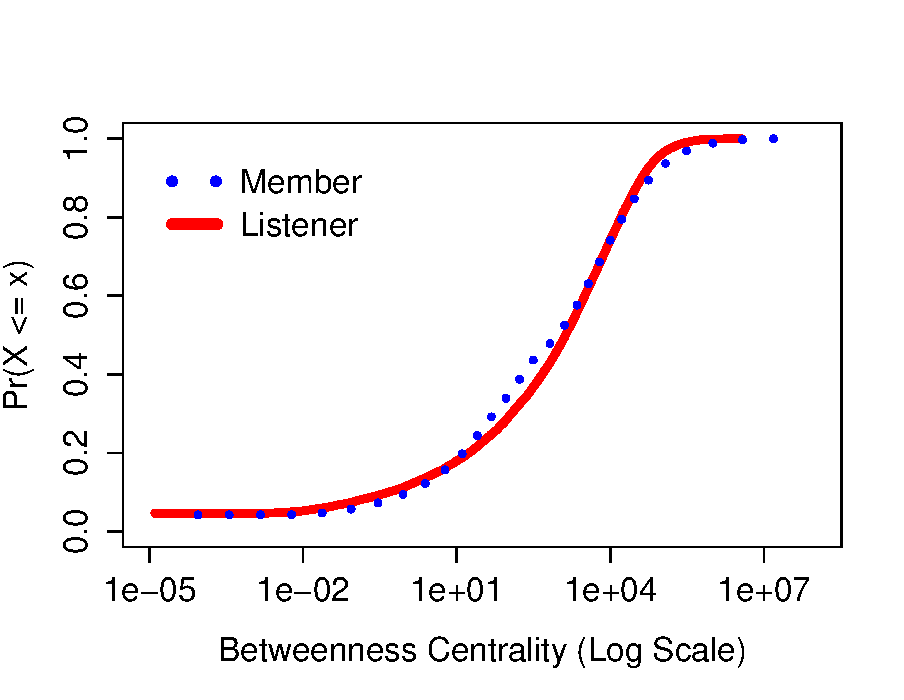
\includegraphics[height=0.4\textwidth]{btcdf.pdf}
		\label{fig:btcdf}}%
	\hfill
	\hspace{-15px}
	\subfloat[]{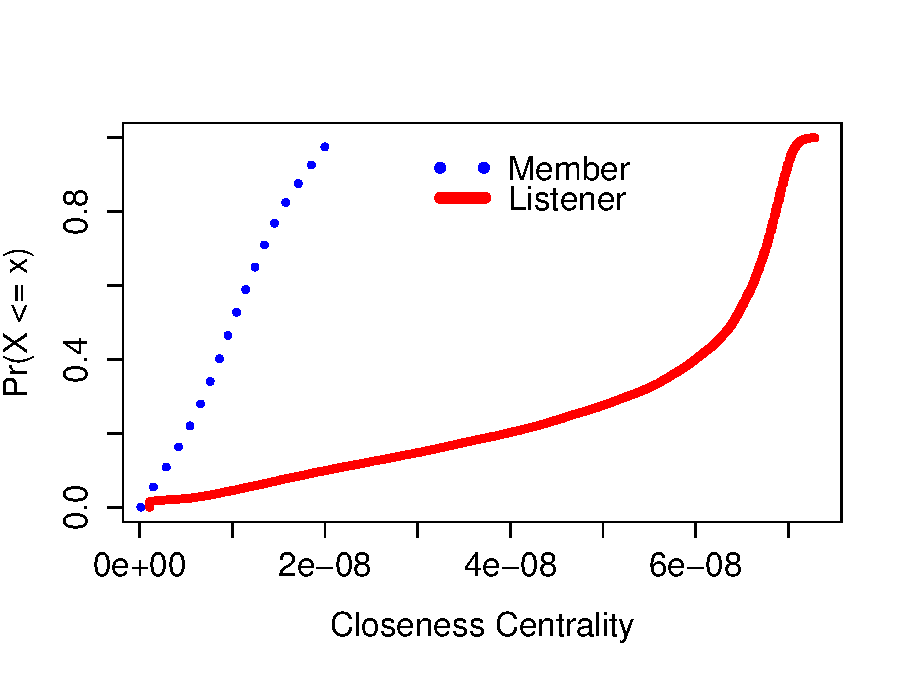
\includegraphics[height=0.4\textwidth]{closecdf.pdf}
		\label{fig:clcdf}}%
	\caption{Centrality distributions for members and listeners}
\end{figure}
%%Here.
\subsection{Network transitivity}
Finally, we use the local clustering coefficient distributions of the projection 
networks to study the tendency of transitive relationships among members
and listeners. A transitive relationship is one where if user $A$ is a 
member (listener) connected to user $B$ and $B$ is connected to $C$, then $A$
is connected to $C$. Table~\ref{tab:proj} lists the global clustering coefficient,
defined as the average of the number of closed triangles in a user's neighborhood 
divided by the number of possible links that could exist within 
it~\cite{watts1998collective}, as $\mathcal{C} = 0.734$ and $0.636$
for the member and listener projections respectively. The large  
coefficients signify that transitive relationships dominate the projection
networks. However, histograms of the local clustering coefficients $\mathcal{C}_l$ in the
member and listener network in Figure~\ref{fig:cc} show that the large values are driven 
by the 38.9\% of members and 13.2\% of listeners whose $\mathcal{C}_l = 1$. The high values
of $\mathcal{C}$ are therefore driven by a small proportion of users with fully
connected neighbors. 
When we consider users whose $\mathcal{C}_l < 1$, 
clustering coefficients appear to be normally distributed.  
Normally distributed $\mathcal{C}_l$ distributions is a typical phenomenon in co-occurrence
networks spanning many systems, including scientific paper authorship~\cite{yang2015defining}, ~\cite{leskovec2007graph}, e-commerce co-purchases~\cite{leskovec2007dynamics}, and ``related page" relationships on search engines~\cite{niu2011zhishi}, but the surge of members where $\mathcal{C}_l = 1$ is 
unique to 7cot interactions. 
%%Rev
This suggests that users with $\mathcal{C}_l = 1$ may not emerge from some natural or 
universal process innate to all co-occurrence networks. This is evidence that 
both members and listeners perform deliberate actions that drive them into fully connected 
neighborhoods in the projection networks. For example, members may be selectively
connecting to the same pool of listeners that may have similar ratings, 
experiences, or bio's suggesting an expertise that members in their neighborhood do.



\begin{figure}[t]
	%   \subfloat[Member projection]{\includegraphics[width=1.74in]{fig/ccvismem.png}}%
	% \hfill
	%   \subfloat[Listener projection]{\includegraphics[width=1.74in]{fig/ccvislist.png}}%
	%   \vfill
	\subfloat[Member projection]{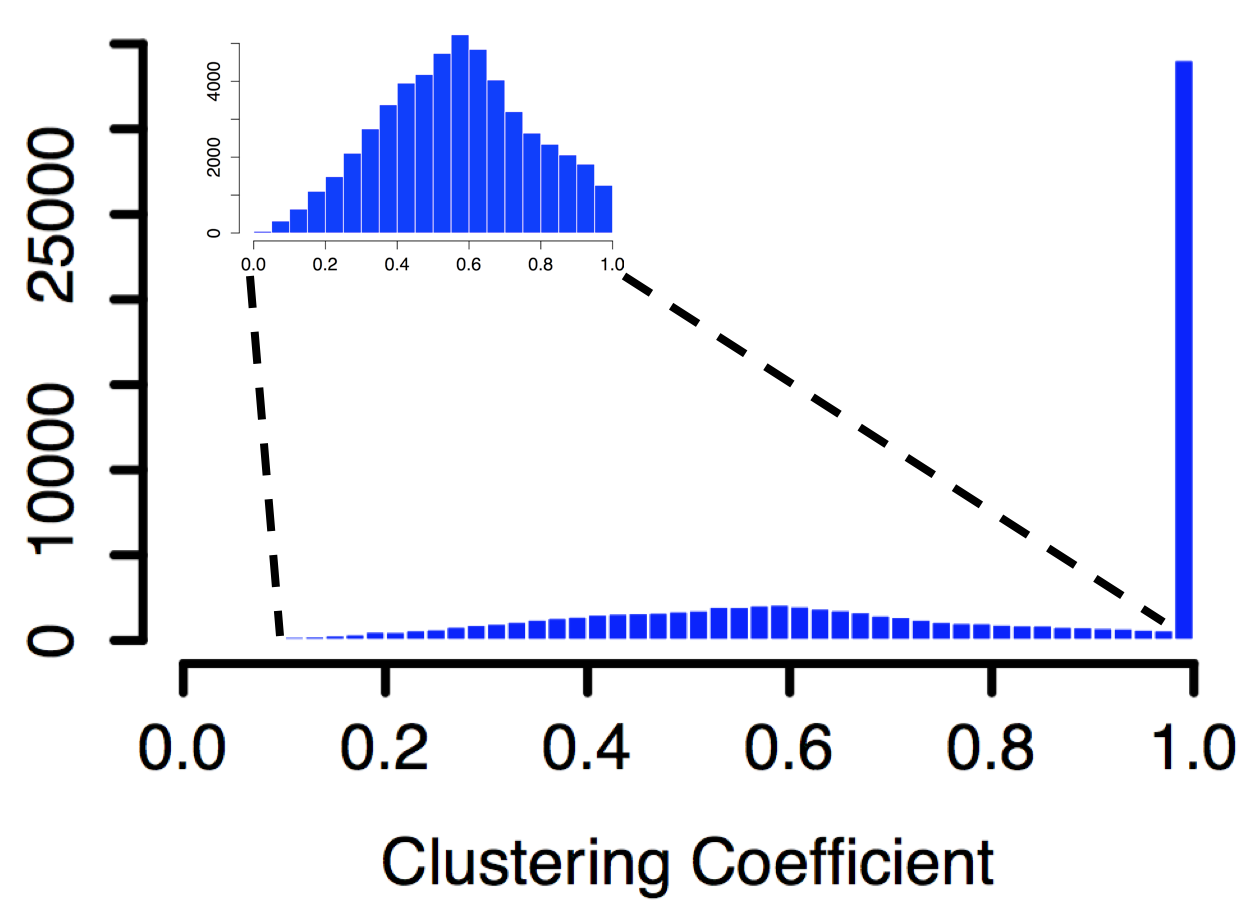
\includegraphics[width=0.45\textwidth]{ccmem2.png}}%
	\hfill
	\subfloat[Listener projection]{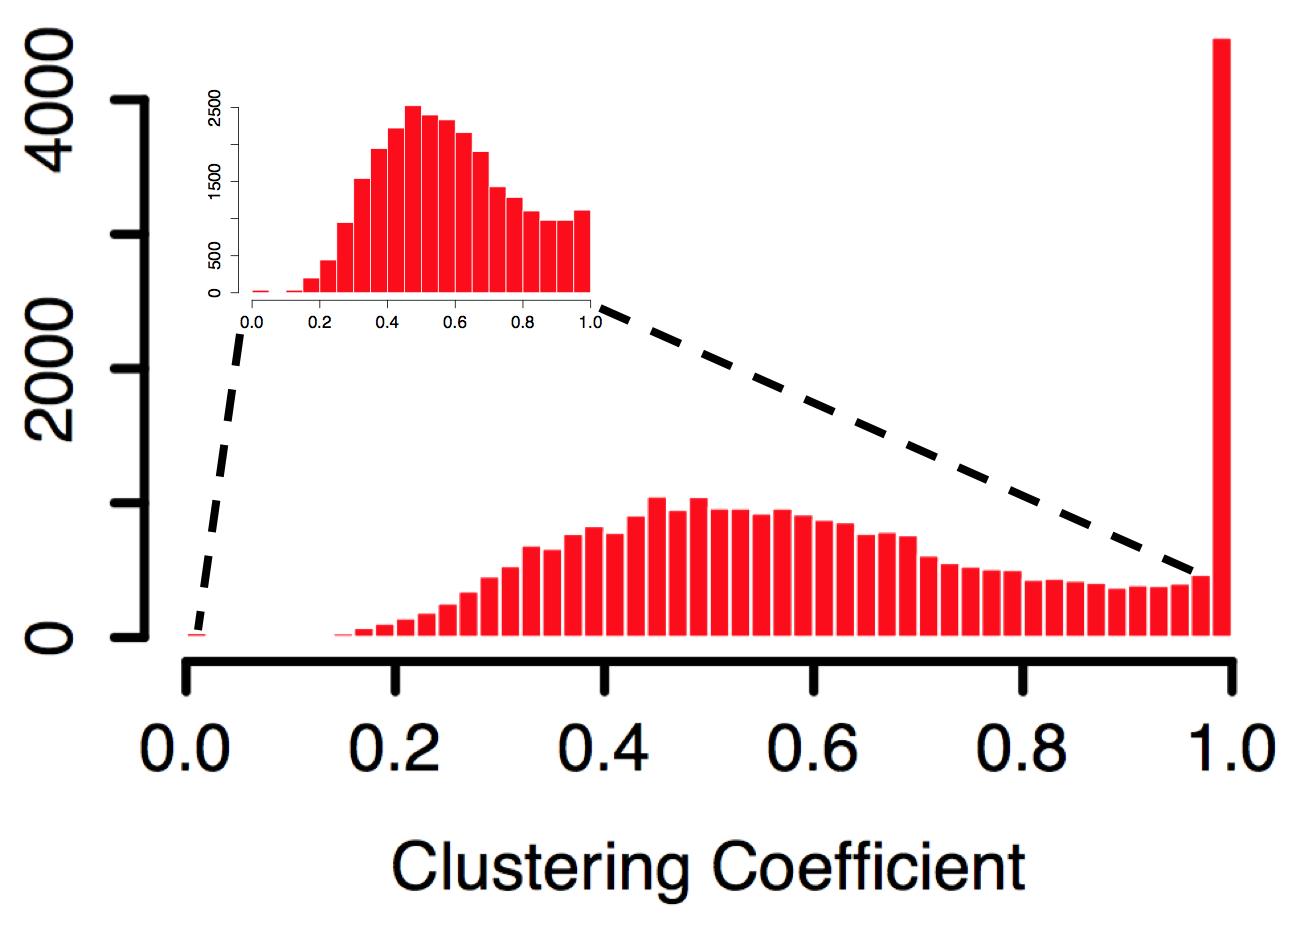
\includegraphics[width=0.45\textwidth]{ccl2.png}}%
	\caption{Projection network cluster coefficient distributions}
	\label{fig:cc}
\end{figure}

\section{Summary of Findings}
In summary, this chapter identified a number of important qualities about the users of 
7cot and the conversations they have. Key takeaways from this study are: 
\begin{itemize}
%	\item Being a registered member on the website has more benefits as compared to being a guest user and therefore could lead to better health outcomes.
%	\item Listeners on the website come from virtually every part of the world, which demonstrates the world wide adoption of this platform and its popularity. Another interesting fact is that, teenagers also tend to use this platform and are comfortable with it. 
%	\item Behavior of some of the users is very anomalous as they seem to be very seasoned and thus making it difficult to say whether heavy tail phenomenon exists on this platform or not.
%	\item The lifetime of members and guest users closely follow double pareto lognormal distribution (DPLN) which the duration of mobile phone calls are known to follow. Preferential attachment holds on this platform.
	\item The giant connected component of the bipartite network include almost all the users of the platform, which tells us that only few users choose to exclusively search for and speak with each other.
	\item The degree distribution of listener projection network follows a power law but same may not be said for the degree distribution of member projection network. This suggest that member may tend to develop deep and strong relationships with some of the listeners rather than having an "exploratory" behavior where they are trying to connect with as many listeners as possible. 
	\item The clustering coefficients of the member and listener projection appears to be normally distributed as is seen in many co-occurrence networks. A small percentage of members and listeners exhibit perfect clustering coefficients which is unique to this platform.
\end{itemize}
%% And now discuss these implications 
